\section{Comparison of Resource Sharing Protocols}
Competition for resources in real-time systems can lead to deadline anomalies. RTOS offers shared memories to different processes, tasks or threads to share computational data among themselves. However, these memories must be accessed exclusively and this is the reason, as it was mentioned before, that the memory areas are guarded by mutex or semaphores~\cite{JiacunWang.2017}.The code segment of the critical section of a task allows it to access the shared data~\cite{JiacunWang.2017}.
\begin{figure}[htbp]
    \centering
    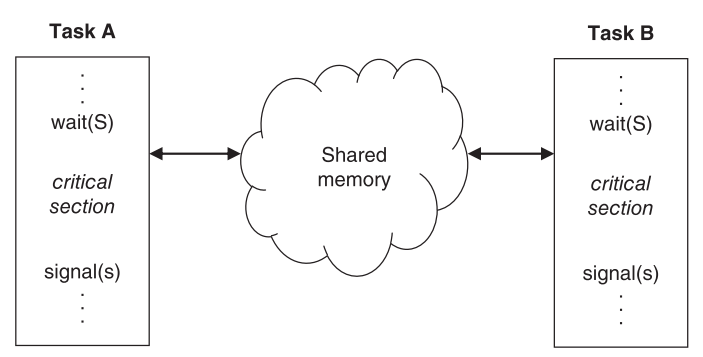
\includegraphics[width=0.95\columnwidth]{Figures/Shared_memory_and_critical_section.png}
    \caption{Shared memory and critical section~\cite{JiacunWang.2017}}\label{fig:Shared_memory_and_critical_section}
\end{figure}
\subsection{Priority Inversion}
Task scheduling is greatly affected by resource sharing and subsequently, when a higher priority task is blocked by a lower priority task- it is known as priority inversion~\cite{JanReineke.2015}.

Priority inversion and deadlocks are major common issues contributing to system failure. Although, there is no protocol that can eliminate priority inversion, the goal of access control is to keep the blocking time of the higher priority tasks under control~\cite{JiacunWang.2017}.\\
For better understanding of how these protocols manage resources allocation among different tasks, a situation can be considered where 3 tasks (J1, J2 and J3) are running in a real-time system. There, are m type of resources in a system, namely R1, R2, R3………, Rm where each resource comprises $\eta_i$ number of indistinguishable units of Ri, i=1, 2, …., m. When a task requests $\rho_i$ units of a resource Ri, request is sent to kernel to lock them and can be denoted as L(Ri, $\rho_i$). When the resource is longer needed by the task, it is unlocked and can be denoted by U(Ri, $\rho_i$). As plentiful resources have no effect on scheduling plentiful resources have no effect on scheduling~\cite{UniversityofGlasgow.}, we can avoid considering them here. Also to be considered here- only the serially reusable resources, which are "one that can be used safely by one task at a time and is not depleted by that use"~\cite{JiacunWang.2017}. The examples of these resources are devices, files, databases, and semaphores~\cite{JiacunWang.2017}. The access to resources by every task will be controlled by locking mechanisms.

Binary semaphores- which are also resources, such as mutexes and suspension-based locks, guarantee mutual exclusion~\cite{dosSantos.2023} by guarding the data  shared between several computational tasks~\cite{JiacunWang.2017}.Semaphore is described by~\cite{Buttazzo.2024} as "Operating systems typically provide a general synchronization tool, called a semaphore, that can be used by tasks to build critical sections. A semaphore is a kernel data structure that, apart from initialization, can be accessed only through two kernel primitives, usually called wait and signal.". A task which is about to enter a critical section must wait until another task, which is having the required resource, releases it~\cite{dosSantos.2023}. As stated by~\cite{Buttazzo.2024} that each critical section, operating on a resource R, must start with a wait(W) primitive and end with a signal(S) primitive. All tasks, blocked on a resource with its semaphore, are put in a queue~\cite{Buttazzo.2024}. The overall mechanisms is described by~\cite{Buttazzo.2024} as- "When a running task executes a wait primitive on a locked semaphore, it enters a waiting state, until another task executes a signal primitive that unlocks the semaphore. When a task leaves the waiting state, it does not go in the running state, but in the ready state, so that the CPU can be assigned to the highest-priority task by the scheduling algorithm."~\cite{Buttazzo.2024}. This is how semaphores protect shared resources in real-time systems by barring concurrent access by multiple tasks.

\begin{figure}[htbp]
    \centering
    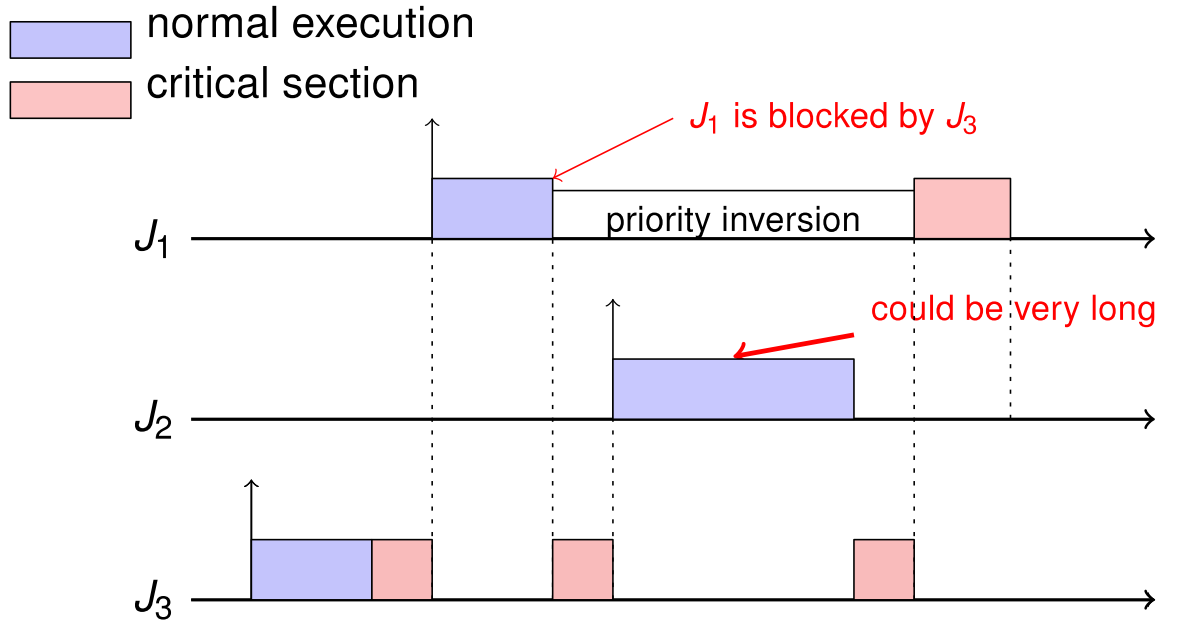
\includegraphics[width=0.95\columnwidth]{Figures/Priority_Inversion_how_it_works.png}
    \caption{Priority inversion and its effects~\cite{JanReineke.2015}}
    \label{fig:Priority_Inversion_how_it_works}
\end{figure}

It can be assumed here, for example, that the task $J_3$ starts at time $t_0$. Task $J_1$ arrives in the system at time $t_2$ and preempts $J_3$ while it is executing inside its critical section since $J_1$ has higher priority. Although, after a while at time $t_3$, when $J_1$ is attempting to start executing at its critical section, it is being blocked on the semaphore and $J_3$ will continue, again, to execute at its critical section. At time $t_4$, yet an another task- '$J_2$' can come at the system, which can preempt $J_3$. Subsequently, the blocking time of $J_1$ is going to prolong one more time. Here, the maximum blocking time of $J_1$ does depend not only on the length of the critical section executed by $J_3$ but also on the worst-case execution time of $J_2$~\cite{Buttazzo.2024}. Thus, priority inversion is said to occur from the moment of $J_1$ being blocked by the semaphore until it once again begins executing. This becomes more complex as any task with intermediate priority can preempt $J_3$ and indirectly blocks $J_1$ for an indefinite time. This is why, "the blocking time of a task on a busy resource cannot be bounded by the duration of the critical section executed by the lower priority task"~\cite{Buttazzo.2024}. This unbounded priority inversion incident can cause the task, blocked on resource access, miss its deadline~\cite{JiacunWang.2017}.\\
\subsection{Deadlock}
Whereas, another phenomenon- deadlock occurs when two or more tasks are waiting for resources to be released by one another, thus creating a cycle of dependencies and situation where none of them can proceed. Deadlock occurs when the following four conditions coincide~\cite{JiacunWang.2017}:
\begin{itemize}
    \item Mutual exclusion: At least one resource must be held in an exclusive mode.
    \item Hold and wait: A task will hold a resource while also waiting for another resource.
    \item No preemption: A resource cannot be forcibly taken from a task holding it.
    \item Circular wait: There must be a set or tasks where each task waits for a resource held by the next task in the set- creating a circular-chain like dependency issue.
\end{itemize}
Let it be considered that there are two tasks- $T_H$ and $T_L$ in a system, where $T_L$ starts executing first. After a short while, it starts using resource A by blocking it. Then, $T_H$ arrives at the system and preempts $T_L$, as $T_H$ has the higher priority. Later, it continues running by taking the resource B, until attempting to lock the resource A. As A is held by $T_L$, $T_H$ gets blocked. Similary, $T_L$, sometime later, when tries to block resource B, it gets blocked. Now both gets blocked from sharing resources as they are held by each other. No task can make progress in this situation.
\begin{figure}[htbp]
    \centering
    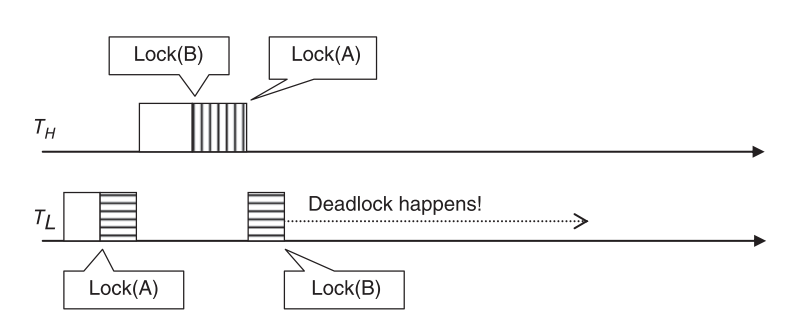
\includegraphics[width=0.95\columnwidth]{Figures/Deadlock.png}
    \caption{Deadlock~\cite{JiacunWang.2017}}\label{fig:Deadlock}
\end{figure}
As it can be seen that resource sharing can cause serious operational problems in real-time systems, there must have to be set of rules to regulate the access to resources by competing tasks. There have been several well-known resource access protocols in place to handle priority inversion and deadlocks efficiently~\cite{JiacunWang.2017}. According to ~\cite{Buttazzo.2024}, the most common protocols are:
\begin{enumerate}[label=\roman*.]
    \item Non-Preemptive Protocol (NPP)
    \item Highest Locker Priority (HLP), also called Immediate Priority Ceiling (IPC);
    \item Priority Inheritance Protocol (PIP)
    \item Priority Ceiling Protocol (PCP)
    \item Stack Resource Policy (SRP)
\end{enumerate}

